\newpage
\section{Nozioni introduttive}
La società moderna è una società digitale. Le immagini passano generalmente per un calcolatore prima di essere stampate, o in ogni caso possono essere sempre scannerizzate (con strumenti più o meno precisi) così da averne una copia digitale.
\`E in questa fase che l'immagine subisce il processo di filtraggio, nel calcolatore, quando è in formato digitale. Per capire cos'è un filtro occorre dunque chiedersi cosa sia un'immagine digitale.

\subsection{Immagini digitali}
\`E necessario comprendere a fondo che cosa sia un oggetto per poterlo successivamente implementare in un calcolatore. A tal scopo è utile quindi capire esattamente che cos'è un'immagine

\begin{quote}
\epigraph{\textit{Forma esteriore degli oggetti corporei, in quanto viene percepita attraverso il senso della vista, o si riflette – come realmente è, o variamente alterata – in uno specchio, nell’acqua e sim., o rimane impressa in una lastra o pellicola o carta fotografica.}}{Vocabolario Treccani}
\end{quote}

\noindent
Un'immagine viene rappresentata impressa su superfici, cioè oggetti bidimensionali, di dimensioni finite la cui visione è resa possibile attraverso i nostri occhi che percepiscono il susseguirsi di diversi colori. Come codificare tali entità?
Come per tutti gli oggetti reali, sebbene questi ultimi abbiano dimensioni finite, le immagini sono distribuzioni continue di colore, o per meglio dire, il susseguirsi delle gradazioni di colore avviene in una maniera che possiamo considerare come continua. La soluzione più largamente utilizzata è anche quella più semplice ed intuitiva, ossia di discretizzare tale distribuzione di colori. Si divide l'immagine con una griglia e ad ogni casella, che d'ora in poi chiameremo \textbf{pixel}, assegnamo un colore.
\`E ovvio che così facendo si perdono dei dettagli, la quantità di dettagli che riusciamo a conservare può variare enormemente, una minima quantità di dettagli si perde sempre ma è un prezzo che vale la pena pagare.
\newpage
Facciamo un esempio:

%\ref{fig:figuraa}. 
\begin{figure}[htb] \centering
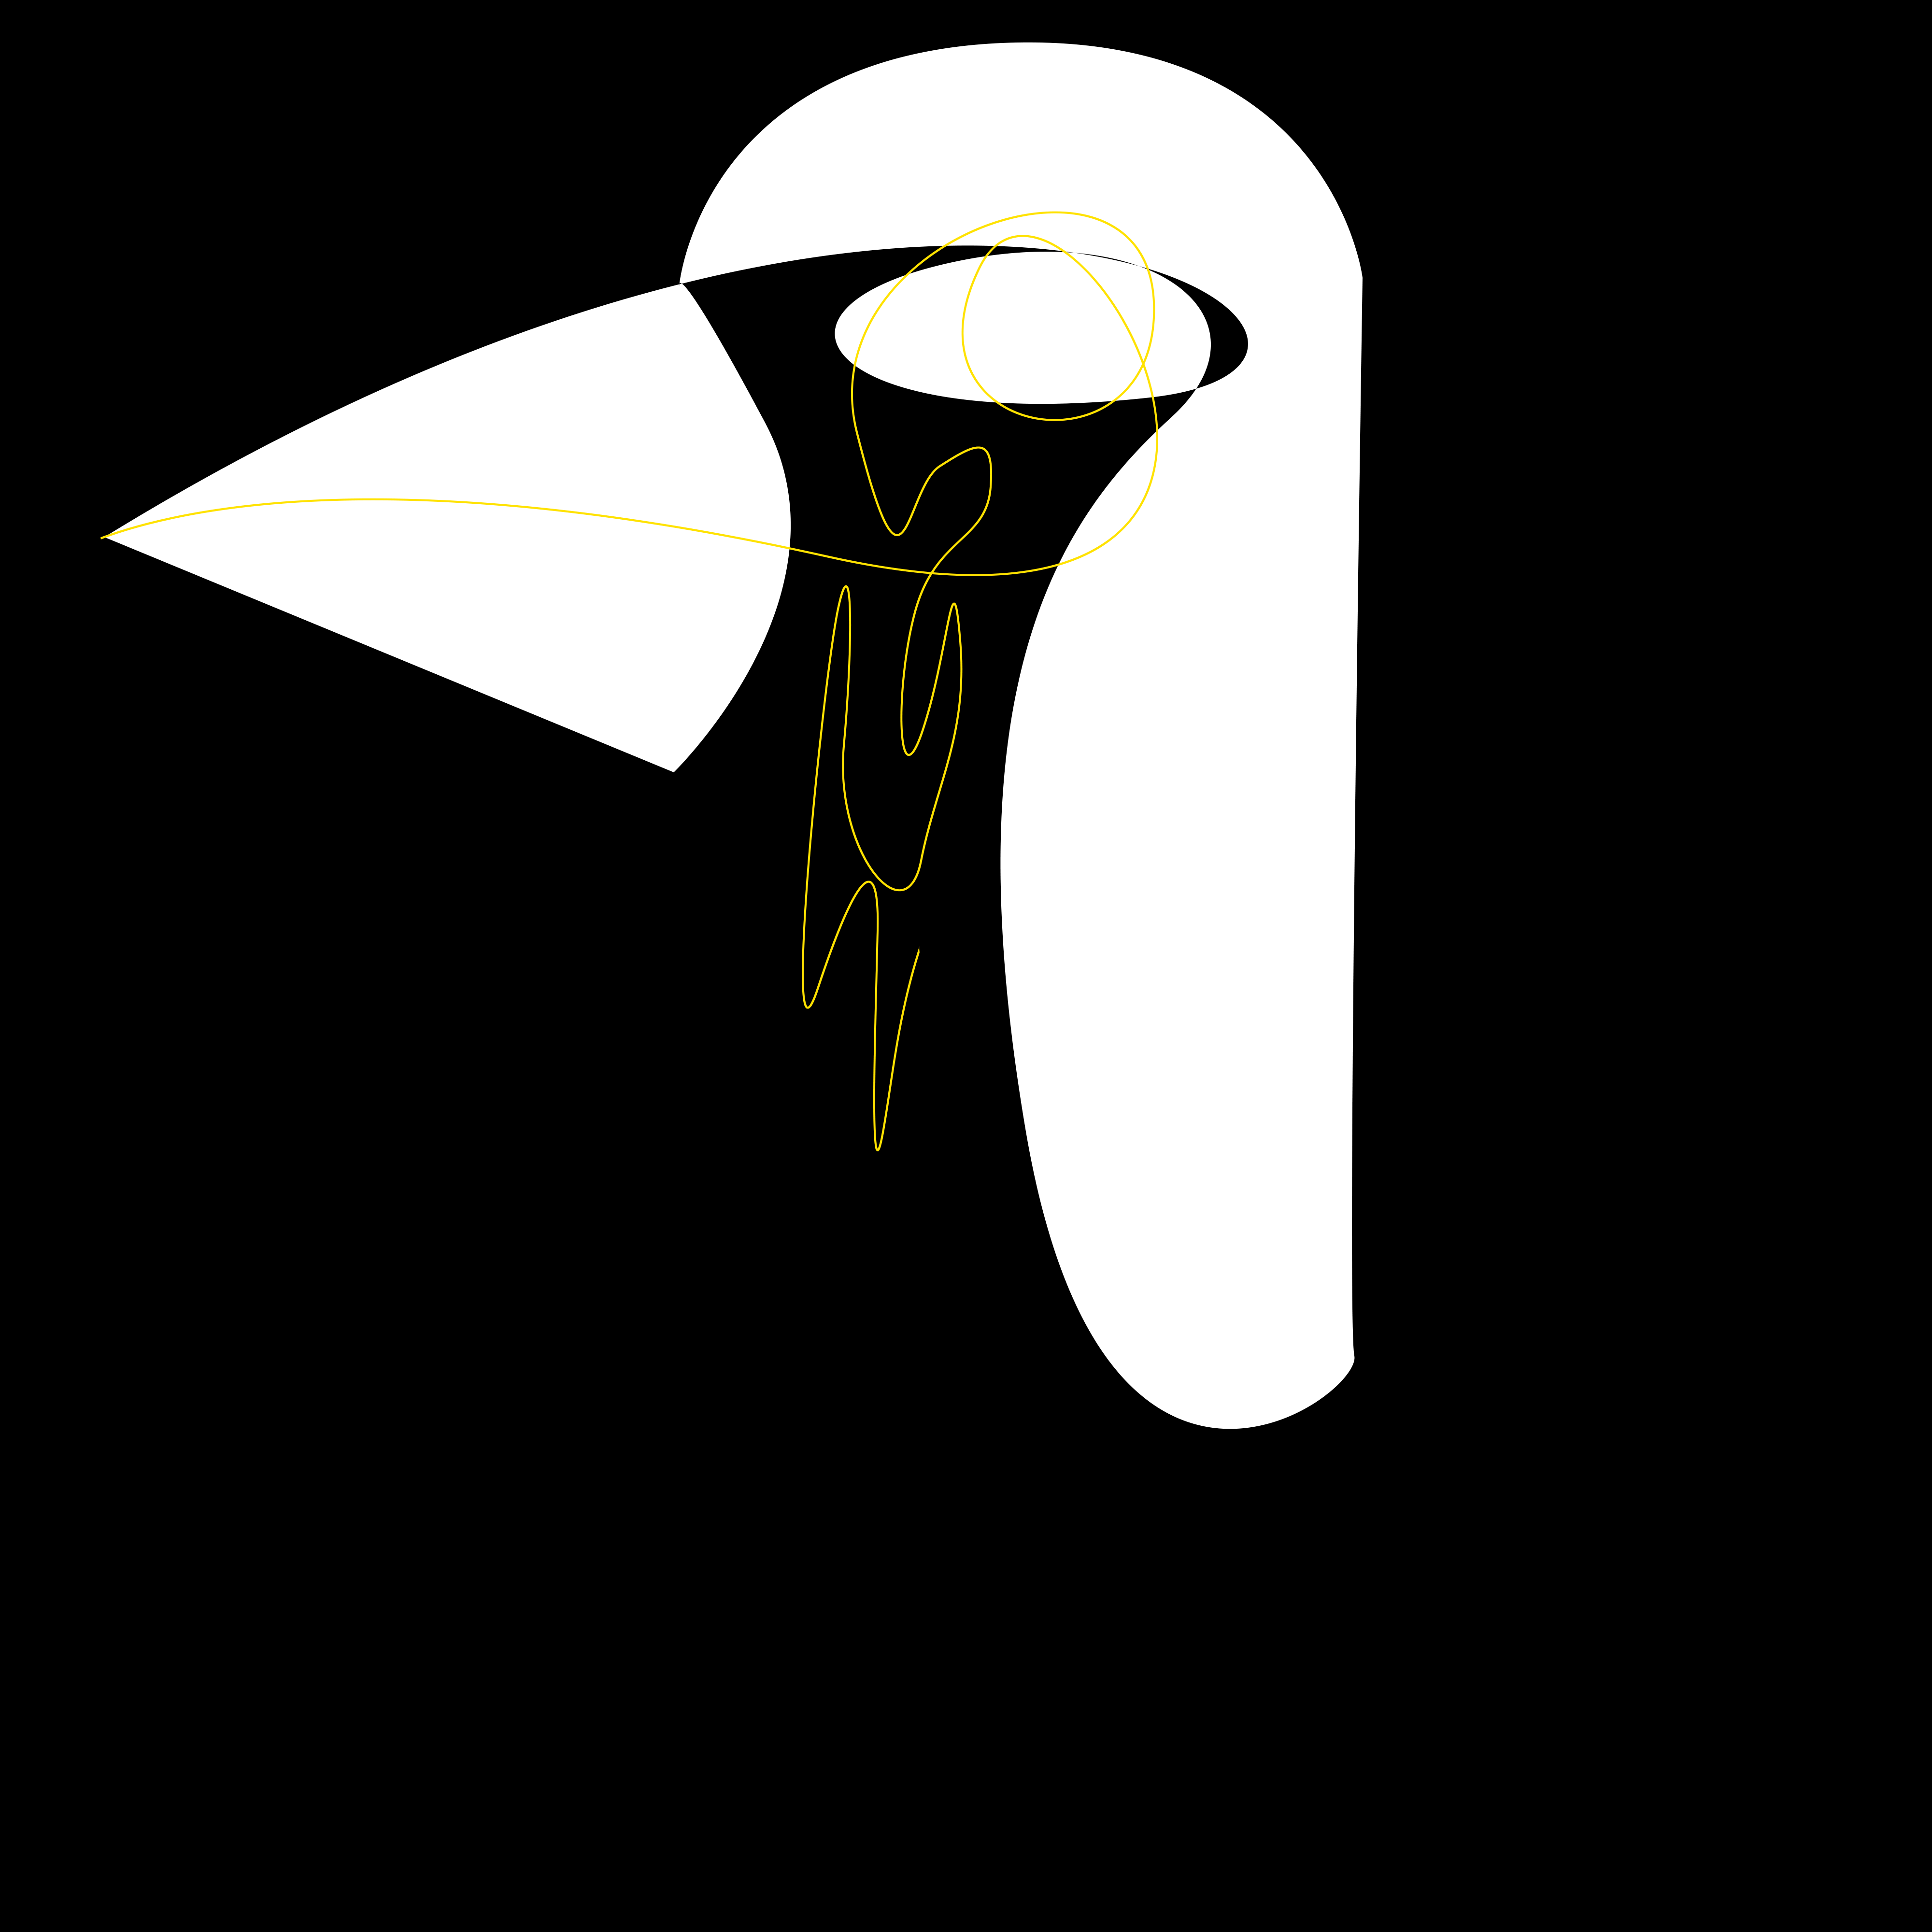
\includegraphics[scale=0.08]{Pictures/in ricordo del pinguino cameriere.png}
%\caption{Fiamme.}\label{fig:figura}
\qquad\qquad

\includegraphics[scale=0.08]{Pictures/canvas8x8.png}
\caption{Confronto tra immagine originale e immagine codificata utilizzando una griglia 4x4.}\label{fig:figura}
\end{figure}

%\ref{fig:figura}. 
\begin{figure}[htb] \centering
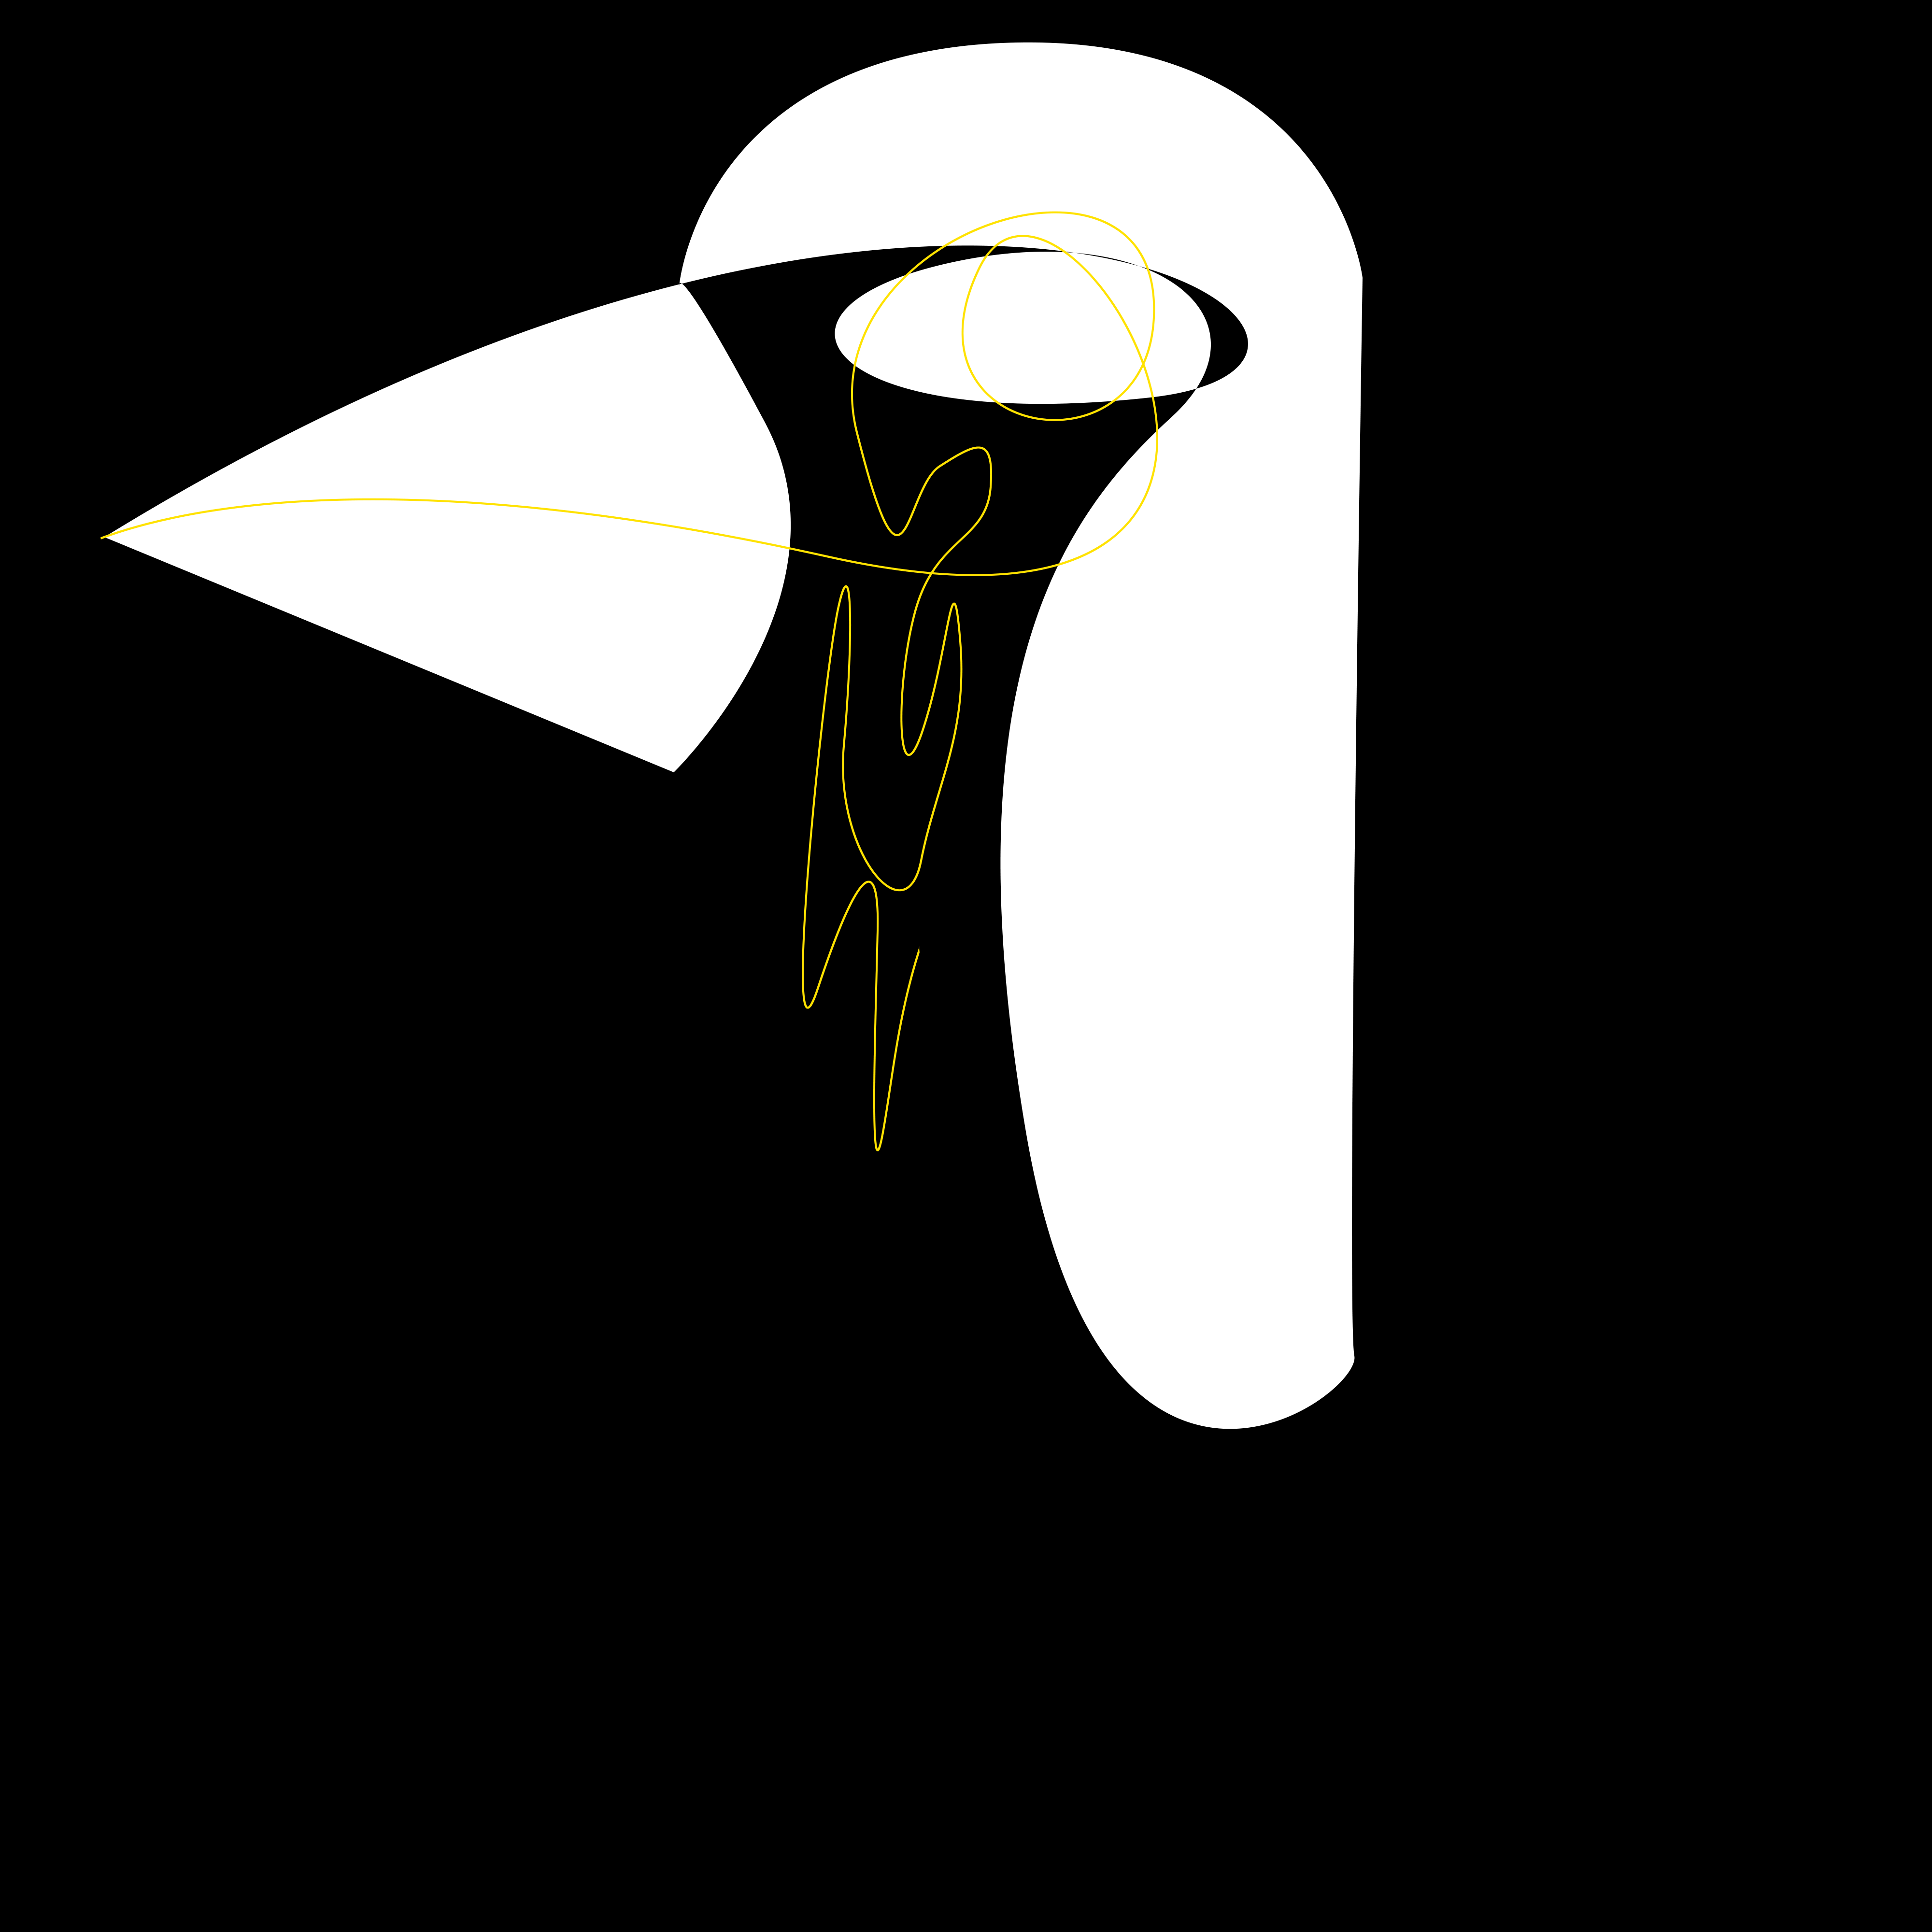
\includegraphics[scale=0.08]{Pictures/in ricordo del pinguino cameriere.png}
\qquad\qquad
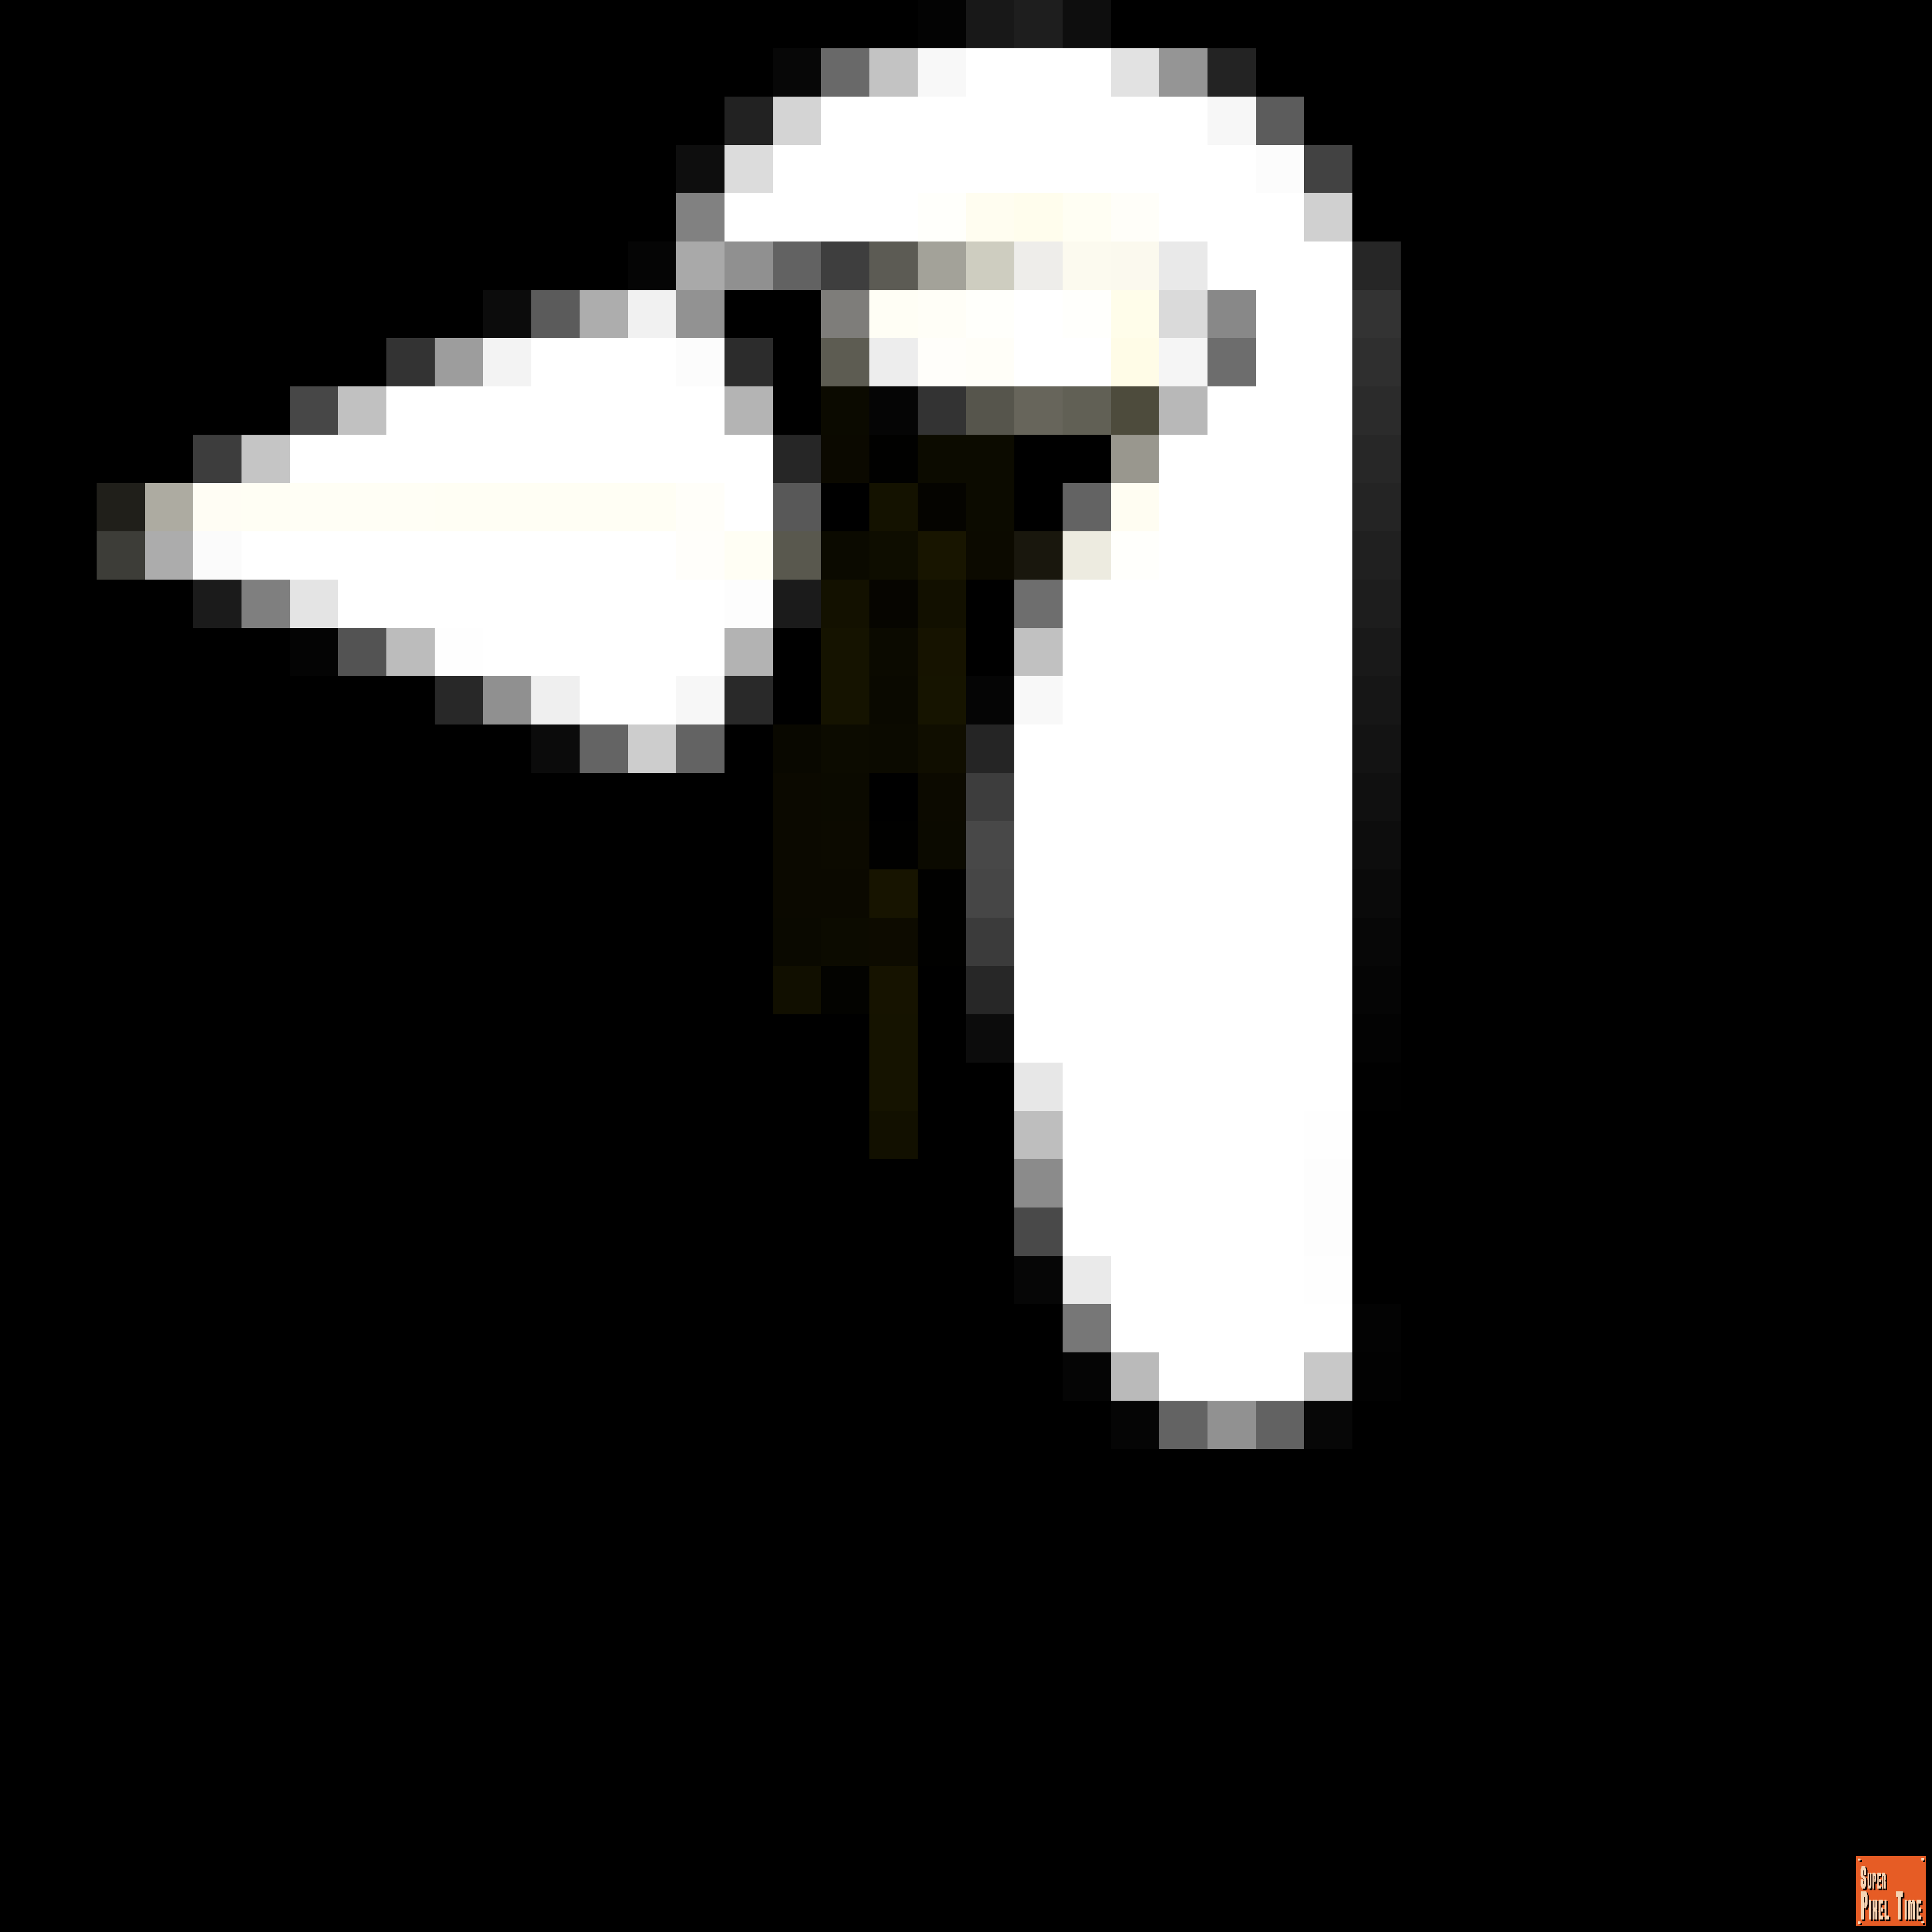
\includegraphics[scale=0.08]{Pictures/canvas80x80.png}
\caption{Confronto tra immagine originale e immagine codificata utilizzando una griglia 80x80.}\label{fig:figura}
\end{figure}

\noindent
\`E semplice vedere come ad una griglia più fitta corrisponda una miglior qualità dell'immagine, questo è il concetto di \textbf{risoluzione di un'immagine}. 
Una miglior risoluzione però costa in termini di memoria. Una griglia 4x4 corrisponde a 16 pixel, ad una griglia 80x80 corrispondono invece 6400 pixel! Questo vuol dire che la seconda immagine pesa 400 volte di più della prima.\\
In particolare se l'immagine è in bianco e nero, per ogni pixel viene occupato 1 bit di memoria, bastano infatti 2 valori: 0 è nero, 1 è bianco. Per memorizzare un'immagine in scala di grigi invece occorrono 8 bit (ossia un byte) per pixel, abbiamo quindi a disposizione 256 valori 0 è nero, 255 è bianco e tutti i numeri naturali tra 1 e 254 rappresentano sfumature di grigio con 1 che rappresenta la gradazione di grigio più scura e 254 la più chiara.  Tornando all'esempio capiamo che formattandola in bianco e nero la prima peserà 2 byte e la seconda 800 byte, formattata in scala di grigi la prima peserà 16 byte mentre la seconda 6.4 chilobyte.  Da questo semplice calcolo capiamo quindi che cambiando tipo di formattazione, per conservare più dettagli, l'occupazione di memoria aumenta parecchio, soprattutto con immagini a grande risoluzione. A riprova di ciò osserviamo che mentre nel passaggio da una risoluzione di 4x4, ad una 80x80 mantenendo la stessa formattazione la seconda è 400 volte più pesante, nel passaggio invece da una risoluzione di 4x4 in bianco e nero ad una di 80x80 in scala di grigi, siccome per ogni pixel serve 1 byte (cioè 8 volte di più di quantoo occorre in bianco e nero), l'aumento sarà quindi $400\cdot8=3200$, cioè la seconda immagine peserà 3200 volte di più della prima.

\vspace{1em} \noindent
Volendo definire in maniera più precisa che cosa è un'immagine digitale, diremmo che quest'ultima è una funzione $u:\mathbb R^2\rightarrow\mathbb R^3$ cioè, date in input due coordinate, essa restituisce un colore (che è formato da 3 canali RGB). Se però l'immagine è in bianco e nero la questione si semplifica: l'immagine diventa una funzione $u:\mathbb R^2\rightarrow\mathbb R$, dal momento che per codificare un colore appartenente alla scala di grigio basta un solo canale: il livello di luminosità. Difatti, la riduzione da tre ad un solo canale rappresenta un grosso vantaggio, permettendo di diminuire di due terzi lo spazio di memoria occupato.
In un'immagine a colori infatti ognuno dei 3 canali è codificato come per la scala di grigi ma sono invece \textit{"scale di rosso, blu e verde"} questo vuol dire che per ogni pixel necessitiamo di 3 byte. Riprendendo ancora una volta l'esempio delle due immagini a bassa ed alta risoluzione, formattate come immagine a colori la prima peserà 48 byte mentre la seconda 19.2 chilobyte. Nel passaggio da una risoluzione di 4x4 in bianco e nero ad una di 80x80 a colori, siccome per ogni pixel servono 3 byte di memoria, l'aumento sarà $400\cdot8\cdot3=9600$, cioè la seconda immagine peserà 9600 volte di più della prima.\\

\subsection{Cosa sono i filtri}
Una volta capito che un'immagine è una funzione possiamo definire un filtro come una seconda funzione $u:\mathbb R^2\rightarrow\mathbb R$ che convoluta alla prima da il risultato richiesto.\\ In matematica, la \textbf{convoluzione} è un'operazione tra due funzioni $f,g \in L^1(X)$ a valori in $\mathbb R$ che consiste nell'integrare il prodotto tra la prima e la seconda traslata di un certo valore, in formule:
$$
h=(f*g)(x)=\int _{X}f(y)g(x-y)\,dy=\int _{X}f(x-y)g(y)\,dy
$$
Si dimostra che $h$ è ancora una funzione $h \in L^1(X)$ a valori in $\mathbb R$.\\
\noindent 
Esistono una varietà di metodi per il filtraggio delle immagini \textbf{basati sulle equazioni alle derivate parziali}. Le equazioni alle derivate parziali (PDE) in generale codificano l'evoluzione di un sistema. Per capire in che modo le PDE possono essere utilizzate per il filtraggio di immagini vediamo un importante risultato per la loro risoluzione.
% prendiamo come esempio l'equazione del calore. 
%$$
%equazione del calore
%$$
\begin{definizione}
Si definisce soluzione fondamentale di un operatore differenziale $L\in \mathcal{D}(\mathbb R^n)$ una distribuzione $u^*$ tale che, $Lu^*=\delta_0$. 
\end{definizione}
\noindent
Trovare la soluzione fondamentale di un operatore differenziale è molto importante nello studio delle equazioni alle derivate parziali siccome, trovata la soluzione fondamentale, siamo in grado di trovare qualsiasi soluzione particolare ci possa interessare, questo grazie a due particolari proprietà dell'operazione di convoluzione. \begin{proposizione}
La prima di cui ci serviremo è: $\forall f\in \mathcal{D}(\mathbb R^n)$, $f*\delta_0=f$.\\
Tale proprietà può essere riassunta con la frase frase \textit{"la $\delta_0$ è l'elemento neutro dell'operazione di convoluzione"}. 
\end{proposizione}
\begin{proposizione}
La seconda proprietà che ci interessa dice che\\ $L(f*g)=L(f)*g=f*L(g)$.
\end{proposizione}
\noindent
Da queste due proprietà discende direttamente che, nota la soluzione fondamentale, la soluzione particolare del problema $Lu=f$ è $u=u^**f$ con $u^*$ soluzione fondamentale di L, infatti $Lu=L(u^**f)=L(u^*)*f=\delta_0*f=f$.\\
\noindent
Questo vuol dire che nel caso $X=\mathbb R^2$ la soluzione fondamentale sarà una funzione definita  $u^*:\mathbb R^2\rightarrow\mathbb R$ e volendo applicare l'operatore differenziale L alla nostra immagine $u_0$ dovremmo fare la convoluzione $u^**u_0$. Parlando in termini di quanto detto ad inizio paragrafo, applicare l'operatore differenziale vuol dire applicare un filtro e il filtro è proprio la soluzione fondamentale dell'operatore.\\
\noindent
Come detto, le PDE codificano un'evoluzione, vedremo infatti che la soluzione di una PDE non dipende solo dai dati iniziali, ma anche da un altro parametro (tipicamente il tempo) che ci aiuterà a regolare in che misura vogliamo che il filtro sia applicato.


%$$u(x)=\frac{1}{w(x)}\int\int d(x-\xi)\Tilde{d}(u_0(x) -u_0(\xi))u_0(\xi)d\xi.$$
%\centering con  $w(x) = \int\int d(x-\xi)\Tilde{d}(u_0(x) -u_0(\xi))d\xi$ \footnote{\cite{korn}}\newline

%\raggedright

\noindent
%E questo è a tutti gli effetti un filtro. 
Il problema adesso è far eseguire questi calcoli ad un calcolatore, il quale non è in grado di lavorare con oggetti continui e richiede quindi di alcune approssimazioni per discretizzare il problema.\\
A tal proposito la definizione di convoluzione può facilmente essere discretizzata parlando di successioni anzichè di funzioni ed operando una sommatoria invece di un integrale.\\
$$
(f*g)[n]\ {\stackrel {{\mathrm {def}}}{=}}\ \sum _{{m=-\infty }}^{\infty }f[m]\,g[n-m]=\sum _{{m=-\infty }}^{\infty }f[n-m]\,g[m].
$$
\noindent
Altri metodi ed approssimazioni saranno poi approfonditi durante la trattazione del problema.

%Definiti questi concetti siamo pronti ad iniziare la trattazione vera e propria

